\documentclass[13pt,addpoints]{exam}
%\usepackage{enumitem}
\usepackage{amsfonts,amssymb,amsmath, amsthm}
\usepackage{graphicx}
\usepackage{systeme}
\usepackage{pgf,tikz,pgfplots}
\pgfplotsset{compat=1.15}
\usepgfplotslibrary{fillbetween}
\usepackage{mathrsfs}
\usetikzlibrary{arrows}
\usetikzlibrary{calc}
\usepackage{geometry}
\geometry{
	a4paper,
	total={170mm,257mm},
	left=20mm,
	top=20mm,
}
\date{December, 2022}
\pagestyle{headandfoot}
%\firstpageheadrule
\runningheader{1st Quarter Midterm Examination}{}{Page \thepage\ of \numpages}
\runningheadrule

\firstpagefooter{}{}{}
\runningfooter{By Aaron G.K.}{}{Page \thepage\ of \numpages}


\begin{document}
	\title{St John Baptist De La Salle Catholic School, Addis Ababa\\
		\large Grade 10 Physics Midterm Examination \\
		$1^\text{st}$ Quarter}
	\maketitle
	\begin{center}
		\fbox{\fbox{\parbox{6in}{\centering
					Notes, and use of other aids is \textbf{NOT} allowed.  Read all directions carefully and \textbf{write your answers in the answer sheet}.  To receive full credit, you must show all of your work.
		}}}
		\subsubsection*{Useful Constants}
	\begin{itemize}
		\item $\textbf{a}_g=10m/s^2\text{  - acceleration due to gravity}$\textbf{~}$\textbf{G} = 6.672\times10^{-12}\frac{Nm^2}{kg^2}\text{  - gravitational constant}$
	\end{itemize}
	
	\end{center}
	{Name:\underline{\hspace{2in}}\text{     }{Roll Number:\underline{\hspace{0.5in}}\text{     }{Section:\underline{\hspace{0.3in}}{Time Allowed: \bf{45  minutes}}
				\subsubsection*{Multiple Choice Questions}
				\begin{questions}
					\question An object rotates at a rate of about 6 rev/min. What is this in revolutions per second? \\
					\begin{oneparchoices}
						\choice 0.1 rev/s
						\choice 12$\pi$rad/s
						\choice 0.1 rad/s
						\choice 6 rev/s
					\end{oneparchoices}
					\question If an object is rotating with a constant angular speed, which of the following is false? \\
					\begin{oneparchoices}
						\choice There is no torque acting on the object.
						\choice The angular acceleration of the object is zero.
						\choice The angular momentum is conserved.
						\choice We don't need to do work to keep the object in rotation.
					\end{oneparchoices}
					\question What is Kepler's Second Law a result of? \\
					\begin{oneparchoices}
						\choice Conservation of Linear Momentum
						\choice Conservation of Charge
						\choice Conservation of Mass
						\choice Conservation of Angular Momentum
					\end{oneparchoices}
					\question The trajectory of planets \& celestial bodies around the sun can't be one of the following geometric shapes: \\ 
					\begin{oneparchoices}
						\choice Ellipse
						\choice Hyperbola
						\choice Lemniscate
						\choice Circle
					\end{oneparchoices}
					\question A point mass the is rotating on the x-axis 1m away from it. If its distance is reduced to 25cm,  by what factor does its moment of inertia change?\\
					\begin{oneparchoices}
						\choice $I_f=\dfrac{1}{4}I_i$
						\choice $I_f=4I_i$
						\choice $I_f=16I_i$
						\choice $I_f=\dfrac{1}{16}I_i$
					\end{oneparchoices}
					\question  When is angular acceleration positive?
					\begin{choices}
						\choice Angular acceleration is the rate of change of the
						displacement and is positive when $\omega$ increases.
						\choice Angular acceleration is the rate of change of the
						displacement and is positive when $\omega$ decreases.
						\choice Angular acceleration is the rate of change of angular
						velocity and is positive when $\omega$ increases.
						\choice Angular acceleration is the rate of change of angular
						velocity and is positive when $\omega$ decreases.
						
					\end{choices}
					\question According to Kepler's Second Law, we do know that the aerial velocity of planets around the sun is constant. Which of the following is  a result of that?
					\begin{choices}
						\choice Planets travel with a constant speed during their trajectory.
						\choice Planets travel faster when they're farthest from the sun and slower when they're near the sun.
						\choice Planets travel faster when they're nearest to the sun and slower when they're farthest from the sun.
						\choice Seasons occur because of this.
					\end{choices}
					\question What did Cavendish measure on the "Weighing the Earth" experiment? \\
					\begin{oneparchoices}
						\choice Weight of the Earth
						\choice Acceleration due to gravity
						\choice Gravitational constant
						\choice Mass of the Earth
					\end{oneparchoices}
					\question When you push a door farther from the hinges, why does it open more fast?
					\begin{choices}
						\choice It opens fast, because the lever arm is shorter so
						the torque is large.
						\choice It opens fast, because the lever arm is longer so the
						torque is large.
						\choice It opens fast, because the lever arm is shorter so
						the torque is less.
						\choice It opens fast, because the lever arm is longer so
						the torque is less.
					\end{choices}
					\question What is the gravitational force between two 70.0 kg
					people sitting $70$ m apart? \\
					\begin{oneparchoices}
						\choice 1 N
						\choice $6.67\times10^{-11}$N
						\choice 70 N
						\choice 0 N
					\end{oneparchoices}
					\subsubsection*{Work Out}
					\question Answer the following questions about angular momentum:
					\begin{itemize}
						\item Show that the torque of a rotating system can be expressed in terms of the time rate of change of the angular momentum.\vspace{0.5in}
						\item If the net torque on a rotating system is 180Nm and it is acted on for 20 seconds, calculate the angular momentum change it causes.\vspace{0.5in}
					\end{itemize}
					\question Consider a CD spinning anticlockwise. What is the sum of the instantaneous velocities of two points on both ends of its diameter?\vspace{0.5in}
					\question Prove Kepler's Third Law.(\textit{For the sake of simplicity, assume the path of planets is circular)}.\vspace{0.9in}
					\question Given that the moon orbits Earth each 27.3 days and that it is an average distance of $3.84\times10^{8}$m from the center of Earth, calculate the period of an artificial satellite orbiting at an average altitude of 1,500 km above Earth’s surface.\vspace{1in}
					\question Let there be a hypothetical planet in our solar system that has an average distance of 2AU from the sun. From your proof above, deduce the period of the planet.(\textit{Note that the period of the Earth is 1 year and it is 1AU away from the sun})\vspace{1in}
				\end{questions}
				\begin{center}
					\subsection*{Answer Sheet}	
				\end{center}	
				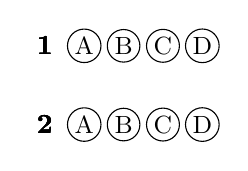
\begin{tikzpicture}[font=\small]
					\foreach \line in {1,2} {
						\begin{scope}[yshift=-\line cm]
							\foreach \letter/\position in {A/1, B/2, C/3, D/4} { 
								\node at (0,0) {\normalsize\textbf{\line}};
								\node[draw,circle,inner sep=1pt] at ({\position * 0.5},0) {\letter};
							}
						\end{scope}
					}
				\end{tikzpicture}\hspace{0.5in}
				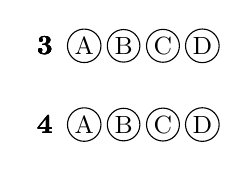
\begin{tikzpicture}[font=\small]
					\foreach \line in {3,4} {
						\begin{scope}[yshift=-\line cm]
							\foreach \letter/\position in {A/1, B/2, C/3, D/4} { 
								\node at (0,0) {\normalsize\textbf{\line}};
								\node[draw,circle,inner sep=1pt] at ({\position * 0.5},0) {\letter};
							}
						\end{scope}
					}
				\end{tikzpicture}\hspace{0.5in}	
				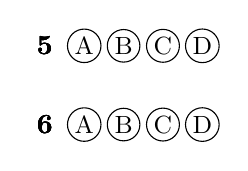
\begin{tikzpicture}[font=\small]
					\foreach \line in {5,6} {
						\begin{scope}[yshift=-\line cm]
							\foreach \letter/\position in {A/1, B/2, C/3, D/4} { 
								\node at (0,0) {\normalsize\textbf{\line}};
								\node[draw,circle,inner sep=1pt] at ({\position * 0.5},0) {\letter};
							}
						\end{scope}
					}
				\end{tikzpicture}\hspace{0.5in}
				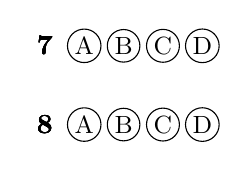
\begin{tikzpicture}[font=\small]
					\foreach \line in {7,8} {
						\begin{scope}[yshift=-\line cm]
							\foreach \letter/\position in {A/1, B/2, C/3, D/4} { 
								\node at (0,0) {\normalsize\textbf{\line}};
								\node[draw,circle,inner sep=1pt] at ({\position * 0.5},0) {\letter};
							}
						\end{scope}
					}
				\end{tikzpicture}\hspace{0.5in}
				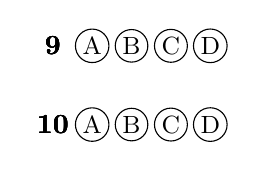
\begin{tikzpicture}[font=\small]
					\foreach \line in {9,10} {
						\begin{scope}[yshift=-\line cm]
							\foreach \letter/\position in {A/1, B/2, C/3, D/4} { 
								\node at (0,0) {\normalsize\textbf{\line}};
								\node[draw,circle,inner sep=1pt] at ({\position * 0.5},0) {\letter};
							}
						\end{scope}
					}
				\end{tikzpicture}	
				
		    \end{document}